\section{Problem}
Når objekters funktionalitet distribueres ud mellem hinanden, vil der opstå høj kobling, og masser af interkonnektivitet.  I et mediator pattern oprettes et separat mediator-objekt, som står for at kontrollere objekters interaktioner med hinanden. 

\section{Løsning}

\begin{figure}[h]
	\centering
	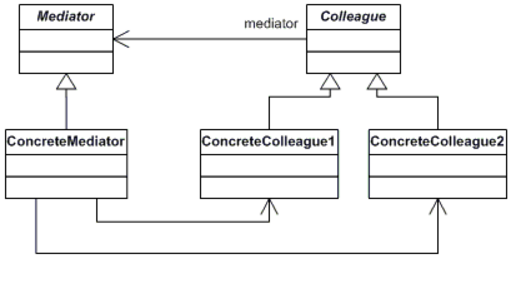
\includegraphics{figs/concrete}
	\caption{}
	\label{fig:concrete}
\end{figure}

Brugen af et mediator pattern begrænser mængden af afledte klasser i et system, i og med mediatoren centraliserer funktionalitet der ellers ville være spredt ud på mange klasser. Ved at pakke objekters interkonnektivitet ind i et mediator pattern, får man samtidig skabt et ekstra abtraktionsniveau der gør funktionalitet mere overskuelig.

\section{Eksempel}
Definition og identifikation af deltagende klassers type:

\begin{itemize}
	\item Mediator.
	\begin{itemize}
		\item 	Definerer et interface til kommunikation with “Colleague objekter”.
	\end{itemize}
	\item Concrete mediator.
	\begin{itemize}
		\item 	Implementerer kommunikationsinterfacet, ved at koordinere Colleague objekter.
	\end{itemize}
	\item Colleague klasser.
	\begin{itemize}
		\item Hver colleague klasse kender sit mediator object.
		\item Når colleaguen vil snakke med en anden klasse, kommunikeres der udelukkende gennem mediatoren.
	\end{itemize}
\end{itemize}

\section{Sammenligning}

\begin{figure}[h]
	\centering
	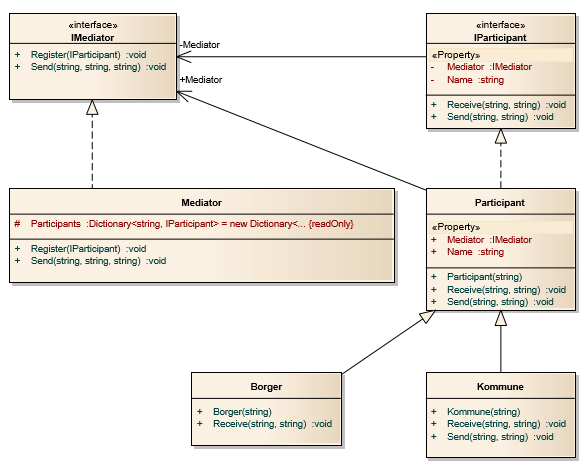
\includegraphics[width=\linewidth]{figs/classdiagram}
	\caption{}
	\label{fig:mediclass}
\end{figure}

\paragraph{Open-Closed}
Mediator pattern mindsker koblingen i programmet. Dette gør, at alle klasser blot skal bruge én reference (til mediatoren), i stedet for at have adskillige referencer til mange forskellige klasser. Dette er godt for Open-Closed princippet, da programmet er åbent for tilføjelser, men lukket for modifikationer. I princippet kan et objekt fjernes fra programmet, uden at programmet går i stykker. Dette skyldes, at mediatoren blot vil undlade at sende en besked, i stedet for, at der er NullPointer referencer i koden.

\paragraph{Single-Responsibility}
SRP betyder, at alle klasser kun skal stå for at udføre én ting, altså have et enkelt ansvar. Derudover skal hver klasse også kun have en grund til at ændre sig. Mediatoren overholder SRP, da dens eneste (og fornemmeste) opgave er at sende beskeder fra A til B, altså at “Mediate”. Selve funktionaliteten der skal udføres, når der modtages en besked ligger ved de individuelle objekter der modtager beskederne fra mediatoren.

\section{Konklusion}